\documentclass[12pt]{report}
\usepackage[fontsize=13pt]{scrextend}
\usepackage[utf8]{vietnam}
\usepackage[utf8]{inputenc}
\usepackage[vietnamese]{babel}
\usepackage{titlesec}
\usepackage{titletoc}
\usepackage{listings}
\usepackage[bookmarks=true]{hyperref}
\usepackage[left=3cm,right=2cm,top=2.5cm,bottom=3cm]{geometry}
\usepackage{graphicx}
\usepackage{hyperref}
\usepackage{tikz}
\usepackage{varwidth}
\usepackage{float}
\usepackage{listings}
\usepackage{color}
\usepackage{multirow}
\usepackage{booktabs}
\usepackage[ruled,vlined]{algorithm2e}
\usepackage{chngcntr}
\usepackage{nameref}
%\usepackage[font=bf]{caption}
%\counterwithin{figure}{chapter}

\renewcommand\labelitemi{--}

\setlength{\parskip}{6pt}

\usetikzlibrary{calc}
\setlength{\parindent}{10mm}
\renewcommand{\baselinestretch}{1.3}
\graphicspath{{images/}}

%%% The following lines add Chapter or Appendix in front of the number
\titlecontents{chapter}%
[0pt]%
{\vspace{1ex}}%
{\bfseries Chương \thecontentslabel\quad}%
{\bfseries}%
{\bfseries\hfill\contentspage}
%%% Initially, for the main part of the document, set the label to "Chapter"
\let\chapappname\chaptername

\definecolor{dkgreen}{rgb}{0,0.6,0}
\definecolor{gray}{rgb}{0.5,0.5,0.5}
\definecolor{mauve}{rgb}{0.58,0,0.82}

% setup code area as listings
\lstset{frame=tb,
  language=Java,
  aboveskip=3mm,
  belowskip=3mm,
  showstringspaces=false,
  columns=flexible,
  basicstyle={\small\ttfamily},
  numbers=left,
  numberstyle=\tiny\color{gray},
  keywordstyle=\color{blue},
  commentstyle=\color{dkgreen},
  stringstyle=\color{mauve},
  breaklines=true,
  breakatwhitespace=true,
  tabsize=3
}

\renewcommand{\lstlistingname}{Mã nguồn}

\newenvironment{thuattoan}[1][h]
  {\renewcommand{\algorithmcfname}{Thuật toán}
   \begin{algorithm}[#1]
  }{\end{algorithm}}

% hyper setup
\hypersetup{
	bookmarks=true,
	pdftitle={Kết hợp bất biến vòng lặp và kỹ thuật thực thi tượng trưng trong kiểm chứng chương trình C/C++},
	pdfauthor={Nguyễn Thị Vân Anh}, % author
	pdfsubject={TeX and LaTeX},
	pdfkeywords={TeX, LaTeX, graphics, images}, % list of keywords
	colorlinks=false,       % false: boxed links; true: colored links
	linkcolor=black,       % color of internal links
	citecolor=black,       % color of links to bibliography
	filecolor=black,        % color of file links
	urlcolor=black,        % color of external links
	linktoc=page            % only page is linked
}

\begin{document}
\begin{titlepage}
	\center
	\begin{tikzpicture}[overlay,remember picture]
		\draw [line width=3pt,rounded corners=0pt,]
		($ (current page.north west) + (25mm,-25mm) $)
		rectangle
		($ (current page.south east) + (-15mm,25mm) $);
		\draw [line width=1pt,rounded corners=0pt]
		($ (current page.north west) + (26.5mm,-26.5mm) $)
		rectangle
		($ (current page.south east) + (-16.5mm,26.5mm) $);
	\end{tikzpicture}
													
	{\large \bfseries ĐẠI HỌC QUỐC GIA HÀ NỘI\\ TRƯỜNG ĐẠI HỌC CÔNG NGHỆ}\\[1cm]
	
\includegraphics[width=0.2\linewidth]{uet}\\[1cm]
		{\Large  \bfseries Nguyễn Tuấn Anh}\\[1.5cm]
		{ \Large \bfseries PHÁT TRIỂN PHẦN MỀM NHẬN DẠNG HOA TRÊN NỀN TẢNG THIẾT BỊ DI ĐỘNG}\\[0.5cm]
		\hfill\\[1.5cm]
		{\large \bfseries KHÓA LUẬN TỐT NGHIỆP ĐẠI HỌC HỆ CHÍNH QUY}\\	
		{\large \bfseries Ngành: Công nghệ thông tin}	
		\hfill\\[3.5cm]	
		{\large \bfseries HÀ NỘI - 2019}\\	
		\vfill
	\end{titlepage}
													
	%-----SECONDARY TITLE PAGE-----%	
	\begin{titlepage}
		\center
		\begin{tikzpicture}[overlay,remember picture]
			\draw [line width=3pt,rounded corners=0pt,]
			($ (current page.north west) + (25mm,-25mm) $)
			rectangle
			($ (current page.south east) + (-15mm,25mm) $);
			\draw [line width=1pt,rounded corners=0pt]
			($ (current page.north west) + (26.5mm,-26.5mm) $)
			rectangle
			($ (current page.south east) + (-16.5mm,26.5mm) $);
		\end{tikzpicture}
																									
		{\large \bfseries ĐẠI HỌC QUỐC GIA HÀ NỘI\\ TRƯỜNG ĐẠI HỌC CÔNG NGHỆ}\\[2cm]
		{\Large  \bfseries Nguyễn Tuấn Anh}\\[2cm]		
		{ \Large \bfseries PHÁT TRIỂN PHẦN MỀM NHẬN DẠNG HOA TRÊN NỀN TẢNG THIẾT BỊ DI ĐỘNG}\\[0.5cm]
		\hfill\\[1.5cm]
		{\large \bfseries KHÓA LUẬN TỐT NGHIỆP ĐẠI HỌC HỆ CHÍNH QUY}\\	
		{\large \bfseries Ngành: Công nghệ thông tin}
		\hfill\\[2cm]
		\begin{flushleft}
			{\large \bfseries Cán bộ hướng dẫn: TS. Nguyễn Thị Ngọc Diệp\\}
																																																		
				\hfill\\[1cm]		
																																																
				{\large \bfseries Cán bộ đồng hướng dẫn: PGS.TS. Nguyễn Việt Hà}\\
																																																		
			\end{flushleft}
			\hfill\\[2cm]		
			{\large \bfseries HÀ NỘI - 2019}\\		
			\vfill		
		\end{titlepage}
																								
		%-----TERTIARY TITLE PAGE-----%	
		\begin{titlepage}
			\center
			\begin{tikzpicture}[overlay,remember picture]
				\draw [line width=3pt,rounded corners=0pt,]
				($ (current page.north west) + (25mm,-25mm) $)
				rectangle
				($ (current page.south east) + (-15mm,25mm) $);
				\draw [line width=1pt,rounded corners=0pt]
				($ (current page.north west) + (26.5mm,-26.5mm) $)
				rectangle
				($ (current page.south east) + (-16.5mm,26.5mm) $);
			\end{tikzpicture}
																																					
			{\large \bfseries VIETNAM NATIONAL UNIVERSITY, HA NOI\\ UNIVERSITY OF ENGINEERING AND TECHNOLOGY}\\[2cm]
																																					
			{\Large  \bfseries Nguyen Tuan Anh}\\[2cm]		
			{ \Large \bfseries DEVELOPING A FLOWER RECOGNITION\\SOFTWARE ON MOBILE DEVICE PLATFORM }\\[0.2cm]
			\hfill\\[1.5cm]
			{\large \bfseries BACHELOR'S THESIS}\\	
			{\large \bfseries Major: Information Technology}
			\hfill\\[3cm]
			\begin{flushleft}
				{\large \bfseries Supervisor: Dr. Nguyen Thi Ngoc Diep }\\
				\hfill\\[1cm]		
																																																		
				{\large \bfseries Co-Supervisor: Assoc. Prof. Nguyen Viet Ha }\\
																																																
			\end{flushleft}
			\hfill\\[2cm]		
			{\large \bfseries HANOI - 2019}\\		
			\vfill		
		\end{titlepage}
																								
		%-----THANKS-----%
		\newpage
		\pagenumbering{roman}
		\begin{center}
			\textbf{\large LỜI CẢM ƠN}
																																					 
																																				
		\end{center}
																								
		Lời đầu tiên cho tôi xin được gửi lời cảm ơn chân thành và sâu sắc nhất tới TS. Nguyễn Thị Ngọc Diệp, PGS. TS. Nguyễn Việt Hà, ThS. Nguyễn Ngọc Khương những người đã hướng dẫn và chỉ bảo tận tình nhất cho tôi trong suốt quá trình hoàn thành khóa luận tốt nghiệp này.
																								
		Tôi xin được gửi lời cảm ơn tới toàn bộ các thầy giáo, cô giáo của trường Đại học Công Nghệ - Đại học Quốc Gia Hà Nội nhưng người đã tạo điều kiện tốt nhất để tôi có thể học tập, nghiên cứu và hơn cả là đã truyền thụ cho tôi những hành trang kiến thức đầy đủ nhất.
																								
		Tôi cũng xin gửi lời cảm ơn chân thành nhất tới các thành viên trong nhóm nghiên cứu SkyLab, tới những người bạn người anh, chị đã giúp đỡ tôi hoàn thiện cả về kiến thức chuyên môn và kỹ năng học tập nghiên cứu.
																								
		Cuối cùng và không thể thiếu đó là lời cảm ơn tới bố mẹ và chị tôi và đặc biệt là bạn Dung Phùng những người đã luôn bên cạnh tôi giúp đỡ và động viên cổ vũ tinh thần tôi trong những lúc khó khăn nhất.
																								
		Tôi xin chân thành cảm ơn!
																								
		\begin{flushright}
			\begin{varwidth}{\linewidth}\centering
				Hà Nội, ngày 24 tháng 04 năm 2019\\
				Sinh viên\\[2cm]
				Nguyễn Tuấn Anh
			\end{varwidth}
		\end{flushright}
																									
		%-----ABSTRACT-----%
		\newpage
		\begin{center}
			\textbf{\large TÓM TẮT}
		\end{center}
																								
		Khóa luận này trình bày một ứng dụng nhận dạng tên loài hoa dựa vào ảnh đầu vào trên nền tảng di động. Ứng dụng này được xây dựng với ba mô hình học máy chính: (1) một mô hình phân loại nhị phân để phát hiện có đối t hoa trong ảnh hay không, (2) một mô hình nhận dạng tên của loài hoa trong ảnh, và (3) một thuật toán tìm kiếm ảnh tương tự khi hiển thị các ảnh kết quả. 
																								
		Ứng dụng được phát triển sử dụng phương pháp sử dụng lại một mô hình học sâu đã được huấn luyện trên bộ dữ liệu lớn khác để trích xuất dữ liệu của ảnh. Thực nghiệm so sánh phương pháp tiếp cận này với các cách trích xuất thuộc tính truyền thống chỉ ra tính khả thi và tiết kiệm của việc sử dụng lại mô hình giữa các bài toán nghiên cứu trong lĩnh vực xử lý ảnh.
																								
		Những đóng góp chính của khóa luận là: (1) Việt hoá tên cũng như đặc điểm về sinh trưởng, cách trồng của 102 loài hoa trong bộ dữ liệu Oxford-102, (2) phát triển ứng dụng trên nền tảng di động, và (3) phát triển mô hình phân loại ảnh có hoa hay không với độ chính xác 98.6\% và mô hình nhận dạng tên loài hoa với độ chính xác là 78.56\%.																			
																								
		\noindent \textit{\textbf{Từ khóa:} nhận diện hoa, phát hiện hoa, ứng dụng di động}
																								
		%-----ABSTRACT (ENGLISH)-----%
		\newpage
		\begin{center}
			\textbf{\large ABSTRACT}
		\end{center}
																								
		This thesis presents an recognition flowers’ names application based on the input images on the mobile platform. This application is built with three main machine learning models: (1) a binary classification model to detect whether there is any flower in the image, (2) a model that recognizes the name of the flower in the image, and (3) an algorithm which searches for results of similar images. 
																								
		The application is developed using a method of reusing a Deep learning models trained by another large data set to extract feature of image. Experimental comparison of this approach with traditional feature extraction method points to the feasibility and savings of reusing model of research problems in the field of image processing.
																								
		The main contributions of this thesis are: (1) Translating names, the growth characteristics as well as planting methods of 102 flower species in Oxford-102 data set, (2) Developing an application on mobile platform, and (3) Developing a flowers detection models with 98.6\% accuracy and an recognition model of flowers with 78.56\% accuracy.
																								
																								
		\noindent \textit{\textbf{Keywords:} flower detection, flower recognition, mobile application}
																								
		%-----UNDERTAKING-----%
		\newpage
		\begin{center}
			\textbf{\large LỜI CAM ĐOAN}
		\end{center}
		Tôi xin cam đoan toàn bộ khóa luận về ứng dụng phát triển phần mềm nhận dạng hoa trên thiết bị di động bao gồm mô hình nhận diện, phần mềm di động và phần mềm hệ thống là do tôi thực hiện dưới sự hướng dẫn của TS. Nguyễn Thị Ngọc Diệp và PGS. TS. Nguyễn Việt Hà. Tất cả các công trình nghiên cứu, bài báo, khóa luận, tài liệu của các tác giả khác được tôi sử dụng trong khóa luận này đều được trích dẫn tường mình về tác giả và đều có trong danh sách tài liệu tham khảo.
																								
		\begin{flushright}
			\begin{varwidth}{\linewidth}\centering
				Hà Nội, ngày 24 tháng 04 năm 2019\\
				Sinh viên\\[2cm]
				Nguyễn Tuấn Anh
			\end{varwidth}
		\end{flushright}
																								
		%-----TOC-----%
		\newpage
		\tableofcontents
																								
		\newpage
		\addcontentsline{toc}{chapter}{\listtablename}
		\listoftables
																								
		\newpage
		\addcontentsline{toc}{chapter}{Danh sách ký hiệu, chữ viết tắt}
		\begin{flushleft}
			\bfseries{\Huge{Danh sách ký hiệu, chữ viết tắt}}
		\end{flushleft}
		\begin{table}[h]
			\centering
			\begin{tabular}{lll}
				\textbf{MRF}       & Markov Random Field                               \\[0.3cm]
				\textbf{HSV}       & Hue, saturation, value                            \\[0.3cm]
				\textbf{SIFT}      & scale-invariant feature transform                 \\[0.3cm]
				\textbf{HOG}       & Histogram of Gradients                            \\[0.3cm]
				\textbf{SVM}       & Support-vector machine                            \\[0.3cm]
				\textbf{SVC}       & Support Vector Classification                     \\[0.3cm]
				\textbf{LinearSVC} & Linear Support Vector Classification              \\[0.3cm]
				\textbf{KNN}       & K-Nearest Neighbour                               \\[0.3cm]
				\textbf{RGB}       & Red, green, blue                                  \\[0.3cm]
				\textbf{CNN}       & Convolutional Neural Network                      \\[0.3cm]
				\textbf{CNNaug}    & Convolutional Neural Network + image augmentation \\[0.3cm]
				\textbf{ONE}       & Online Nearest-neighbor Estimation                \\[0.3cm]
				\textbf{PCA}       & Principal Component Analysis                      \\[0.3cm]
																																																		
			\end{tabular}
		\end{table}
																								
		\newpage
		\addcontentsline{toc}{chapter}{\listfigurename}
		\listoffigures
																								
		%-----MAIN-----%
		\newpage
		\pagenumbering{arabic}
		\setcounter{page}{1}
		\chapter{Mở đầu}
		\label{chap:intro}
																								
		\section{Bối cảnh nghiên cứu}
																								
		Cùng với sự phát triển của công nghệ nói chung cũng như sự phát triển của các thiết bị di động nói riêng ta có thể nhận thấy một điều rằng ngày nay điện thoại di động là một dụng cụ luôn đi kèm mỗi người mỗi khi đi ra khỏi nhà, đi làm hay đi chơi. Một ví dụ như sau trong một lần đi dạo bạn bỗng nhìn một bông hoa rất đẹp trồng ở ven đường và tự hỏi tên của loài hoa đó là gì. Bạn thấy rằng bông hoa đó rất quen thuộc nhưng không thể nhớ ra được. Bạn nghĩ ngay tới việc tìm kiếm trên Google và có thử lấy điện thoại di động của mình ra chụp ảnh bông hoa đó và tìm trên Google nhưng không thật không may các kết quả tìm kiếm chỉ là các hình ảnh tương tự với ảnh mà bạn chụp và tên các loài hoa thì toàn là tiếng Anh và tiếng Latin, không những thế đôi khi các kết quả trả về từ Google lại không hề liên quan tới tên loài hoa đó.
		Qua ví dụ trên ta có thể nhận thấy nhu cầu về tìm kiếm tên của các loài hoa từ ảnh chụp thực tế từ các thiết bị di động là hoàn toàn có cơ sở. Do vậy cần một ứng dụng có chức năng nhận dạng tên loài hoa từ các ảnh chụp trên thiết bị di động.
																								
		\begin{figure}[h]
			\centering
			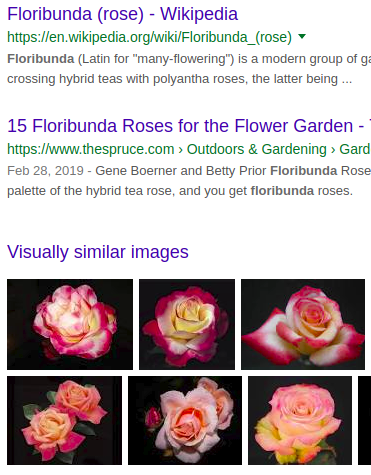
\includegraphics[scale=0.6]{anh_1}
			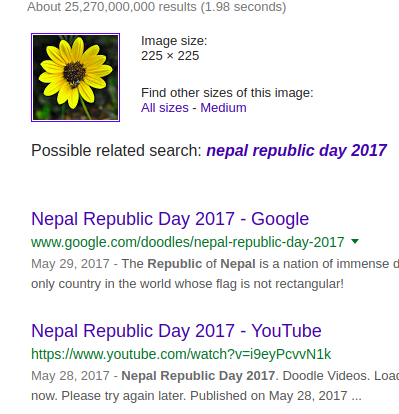
\includegraphics[scale=0.6]{anh_2}
																																				
			\caption{Ví dụ về tìm kiếm hình ảnh của Google Images}
			\label{fig:anh_1}
		\end{figure}
																								
		\section{Mô tả bài toán nhận dạng hoa}
		Mô tả bài toán: bài toán nhận dạng hoa thông qua ảnh chụp sẽ có đầu vào là một hình ảnh được ghi lại từ các thiết bị ghi hình và đầu ra có thể có hai trường hợp
		\begin{itemize}
			\item \texttt{Trường hợp 1:} Trong ảnh không có hoa thì kết quả trả về là không tồn tại hoa.
			\item \texttt{Trường hợp 2:} Trong ảnh có hoa thì kết quả trả về là một danh sách 5 loài hoa có kết quả nhận dạng tốt nhất.
		\end{itemize}
		Những khó khăn khi nhận diện hoa
		\begin{itemize}
			\item  Số lượng các loài hoa khác nhau mọc trong tự nhiên vô cùng đa dạng và phong phú. Các loài hoa có vô số màu sắc, kiểu dáng hình thù khác nhau gây khó khăn khi phải phân loại với một số lượng loài lớn.
			\item  Các loài hoa đôi khi có kiểu dáng tương đối giống nhau.
			\item  Các loài hoa trong thời gian sinh trưởng có rất nhiều hình thái khác nhau gây ra nhầm lẫn một ví dụ điển hình có thể thấy đó là hoa sen khi chưa nở và lúc đã nở có hình dạng rất khác nhau.
		\end{itemize}
																								
		\begin{figure}[h]
			\centering
			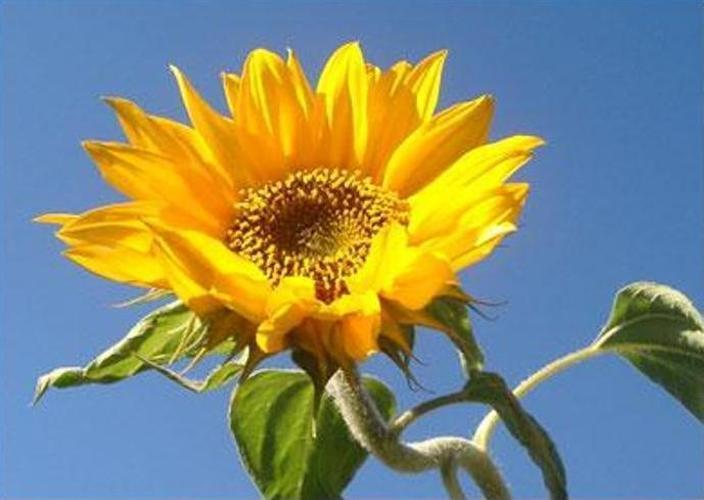
\includegraphics[scale=0.3]{anh_4}
			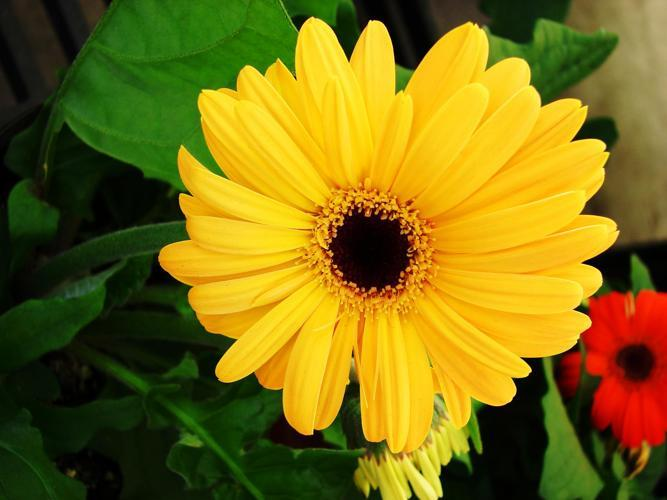
\includegraphics[scale=0.3]{anh_3}
			\caption{Hình ảnh ví dụ về các loài hoa có cấu trúc giống nhau}
			\label{fig:anh_1}
		\end{figure}
		(Ở bên trái là ảnh hoa hướng dương còn ở bên phải là ảnh hoa cúc)
																						
		\begin{figure}[h]
			\centering
			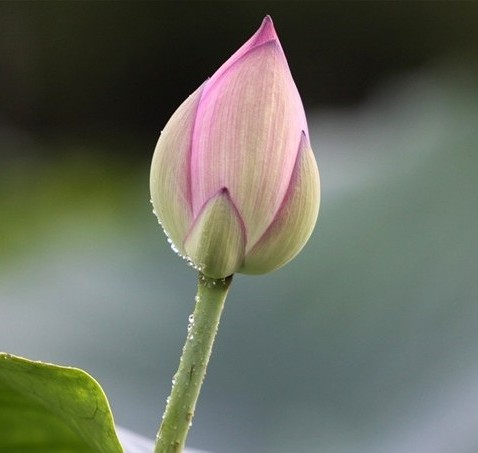
\includegraphics[scale=0.4]{anh_5}
			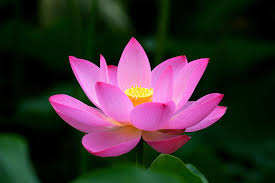
\includegraphics[scale=0.9]{anh_6}
			\caption{Hình ảnh ví dụ về các loài hoa thay đổi hình dạng theo thời gian}
			\label{fig:anh_1}
		\end{figure}
		(Ở bên trái là ảnh hoa sen khi chưa nở còn ở bên phải là ảnh hoa sen khi đã nở)
																								
		\section{Mục tiêu và phương pháp giải quyết vấn đề}
		\subsection{Mục tiêu của khóa luận}
																						
		Mục đích chính của khóa luận này muốn nhắm tới đó là phát triển một ứng dụng nhận dạng tên các loài hoa dành cho người Việt trên nền tảng thiết bị di động. Qua đó cũng đề xuất phương pháp sử dụng mạng học sâu đã được huấn luyện VGG19 [16] trong các mô hình trích xuất thuộc tính từ ảnh, đồng thời tạo tiền đề phát triển cho những nghiên cứu sau này về đề tài nhận diện ảnh.
																				
		Ứng dụng sau khi được phát triển sẽ không đơn thuần chỉ là một công cụ tra cứu mà còn có ý nghĩa trở thành một công cụ học tập, nghiên cứu về thiên nhiên và đặc biệt là các loài hoa giúp các em học sinh, mọi người ở mọi lứa tuổi có thêm một công cụ hữu ích trong việc học tập và nghiên cứu về các loài hoa.
																				
		\subsection{Phương pháp giải quyết bài toán nhận dạng hoa}
																		
		Để giải quyết được bài toán nhận dạng tên loài hoa sử dụng ảnh ta cần phải qua năm bước chính đó là:
																		
		\begin{itemize}
			\item \texttt{Bước 1:} Tiền xử lý dữ liệu hình ảnh.
			\item \texttt{Bước 2:} Trích xuất các thuộc tính từ ảnh và chuyển thành các vector thuộc tính.
			\item \texttt{Bước 3:} Sử dụng các thuật toán phân loại để phát hiện có hoa trong ảnh hay không.
			\item \texttt{Bước 4:}	Nếu phát hiện thấy hoa trong ảnh thì sử dụng vector thuộc tính đó để nhận dạng tên loài hoa
			\item \texttt{Bước 5}: Tính toán độ tương tự của các ảnh trong tưng loài hoa để đưa ra các ảnh phù hợp nhất cho kết quả.
		\end{itemize}
																
		Qua sự tham khảo các phương pháp trích xuất truyền thống như đã được công bố trong các nghiên cứu [1] [2] và các nghiên cứu gần đây sử dụng mạng tích chập VGG19 [16]. Phương pháp để giải quyết bài toán sẽ diễn ra với các bước sau:
																
		\begin{itemize}
			\item Tiền xử lý hình ảnh bằng phương pháp tách phông nền.
			\item Trích xuất thuộc tính của ảnh sử dụng mạng VGG19 [16]
			\item Xây dựng một mô hình phân loại nhị phân dùng để phát hiện có đối tượng hoa trong ảnh hay không.
			\item Xây dựng một mô hình nhận dạng tên của loài hoa trong ảnh.
			\item Và cuối cùng là một thuật toán tìm kiếm ảnh tương tự khi hiển thị các ảnh kết quả.
		\end{itemize}
										
										
		\subsection{Những điểm mạnh của phương pháp này}
		Qua thực nghiệm và so sánh phương pháp trích xuất thuộc tính sử dụng mô hình học sâu VGG19 [16] với các cách trích xuất thuộc tính truyền thống có kết quả khá khả quan và có tính khả thi cao.
						
		Hơn nữa việc sử dụng lại mô hình trích xuất thuộc tính giữa các bài toán nhận dạng sẽ tiết kiệm được đáng kể công sức cũng như cải thiện được độ chính xác phân loại.
						
		\section{Bố cục các phần trong khóa luận}
		Các phần trong khóa luận được cấu trúc như sau.
						
				
		\begin{itemize}
			\item \textbf{Chương \ref{chap:intro}}: Giới thiệu về bài toán nhận dạng hoa, mục đích và các phương pháp sử dụng để giải quyết bài toán phát triển ứng dụng nhận dạng hoa trên thiết bị di động.
			\item \textbf{Chương \ref{chap:background}}: Trình bày các nghiên cứu liên quan đến bài toán nhận dạng hoa. Các phương pháp trích xuất thuộc tính truyền thống và các phương pháp mới sử dụng mạng học sâu.
			\item \textbf{Chương \ref{chap:solution}}: Trình bày và giải thích về mô hình tổng quát của ứng dụng cũng như cách huấn luyện các mô hình phân loại được sử dụng trong hệ thống.
			\item \textbf{Chương \ref{chap:Experimental results}}: Mô tả về cách thu thập dữ liệu, cách cài đặt và sử dụng các thuật toán để giải quyết vấn đề đồng thời giải thích về mục đích cũng như đưa ra các số liệu thống kê về các kết quả đã đạt được trong từng thí nghiệm. 
			\item \textbf{Chương \ref{chap:conclusion}}: Đưa ra các kết luận về những vấn đề đã giải quyết và những vấn đề chưa giải quyết được đồng thời giới thiệu hướng nghiên cứu để tiếp tục phát triển trong tương lai.	      
		\end{itemize}
						
		
				
				
		% chương 2
		\newpage	
		\chapter{Nghiên cứu liên quan đến bài toán nhận dạng hoa}
		\label{chap:background}
								
										
		\section{Các bộ dữ liệu hoa}
		Có khá nhiều các bộ dữ liệu về hoa nổi tiếng và đa dạng ta có thể kể đến như	
		\begin{itemize}
			\item Bộ dữ liệu về hoa của ImageNet.
			\item Oxford-17 [1] bao gồm 1360 ảnh thuộc 17 loài hoa.
			\item Oxford-102 [1] bao gồm 8189 ảnh thuộc 102 loài hoa. 
			\item Kaggle flower dataset: bao gồm 4242 ảnh của 5 loài hoa.
			\item Bộ dữ liệu về thực vật trên trang plant database https://garden.org/plants/.
		\end{itemize}		
						
		Trong khóa luận này sử dụng bộ dữ liệu hoa Oxford-102 [1], vì các lý do sau.
		
		\begin{itemize}
			\item Số lượng loài nhiều, số lượng ảnh mỗi loài cũng nhiều.
			\item Các ảnh chụp đều là ảnh chụp cận cảnh bông hoa và đa dạng về góc chụp, ánh sáng.
			\item Các ảnh mỗi loài đều có số lượng loại phong phú, ví dụ ở đây hoa hồng có cả đỏ, hồng, trắng.. thay vì chỉ một loại hoa hồng đỏ.
			\item Có nhiều nghiên cứu sử dụng bộ dữ liệu Oxford-102 \cite{cia-Nilsback06}, cụ thể trong khóa luận có đề cập tới 4 nghiên cứu [1] [2] [3] [4].
		\end{itemize}				
						
		Bộ dữ liệu đã được chia thành bộ huấn luyện bao gồm 10 ảnh mỗi loài hoa, bộ xác nhận bao gồm 10 ảnh mỗi loại và các ảnh còn lại gồm 6129 ảnh làm bộ kiểm tra. 	
						
		% chương 3
		\newpage
		\chapter{Phát triển phần mềm nhận dạng hoa trên thiết bị di động}
		\label{chap:solution}
		\section{}
										
						
						
						
						
						
						
						
						
						
		% chương 4													
		\chapter{Kết quả thực nghiệm}
		\label{chap:Experimental results}
										
		% chương 5
		\chapter{Kết luận}
		\label{chap:conclusion}
										
		Trong khóa luận này trình bày một ứng dụng nhận dạng tên loài hoa dựa vào ảnh đầu vào trên nền tảng di động. Ứng dụng này được xây dựng với ba mô hình học máy chính: (1) một mô hình phân loại nhị phân để phát hiện có đối tượng hoa trong ảnh hay không, (2) một mô hình nhận dạng tên của loài hoa trong ảnh, và (3) một thuật toán tìm kiếm ảnh tương tự khi hiển thị các ảnh kết quả. 
										
		Ứng dụng được phát triển sử dụng phương pháp sử dụng lại một mô hình học sâu đã được huấn luyện trên bộ dữ liệu lớn khác để trích xuất dữ liệu của ảnh VGG19 [16]. Thực nghiệm so sánh phương pháp tiếp cận này với các cách trích xuất thuộc tính truyền thống chỉ ra tính khả thi và tiết kiệm của việc sử dụng lại mô hình giữa các bài toán nghiên cứu trong lĩnh vực xử lý ảnh.
										
		Những đóng góp chính của khóa luận là: (1) Việt hoá tên cũng như đặc điểm về sinh trưởng, cách trồng của 102 loài hoa trong bộ dữ liệu Oxford-102, (2) phát triển ứng dụng trên nền tảng di động, và (3) phát triển mô hình phân loại ảnh có hoa hay không với độ chính xác 98.6\% và mô hình nhận dạng tên loài hoa với độ chính xác là 78.56\%.
										
		Hướng phát triển tiếp theo của nghiên cứu là  tìm cách khắc phục các điểm còn hạn chế trong việc nhận dạng hoa như nhận dạng đa chủ thể hoa hay nhận dạng hoa khi mọc cả chùm.															
																								
		\begin{thebibliography}{9}
																								
			\section*{Tiếng Anh}
																					
			\bibitem{cia-Nilsback06} 
			Maria-Elena Nilsback and Andrew Zisserman. A Visual Vocabulary for Flower Classification Robotics Research Group, Department of Engineering Science University of Oxford, United Kingdom													
																								
			\bibitem{cia-Nilsback08}
			Maria-Elena Nilsback and Andrew Zisserman. Automated flower classification over a large number of classes Visual Geometry Group, Department of Engineering Science University of Oxford, United Kingdom
																					
			\bibitem{cia-ONE}
			Lingxi Xie , Richang Hong , Bo Zhang , and Qi Tian. Image Classification and Retrieval are ONE
																					
			\bibitem{cia-CNNFeatures off-the-shelf}
			CNN Features off-the-shelf: an Astounding Baseline for Recognition Ali Sharif Razavian Hossein Azizpour Josephine Sullivan Stefan Carlsson CVAP, KTH (Royal Institute of Technology) Stockholm, Sweden
																				
			\bibitem{cia_5}
			M. Varma and D. Ray. Learning the discriminative power invariance trade-off. In Proc. ICCV, 2007.
															
			\bibitem{cia_SIFT}
			D. Lowe. Distinctive image features from scale-invariant keypoints. IJCV, 60(2):91–110, 2004.
																							
			\bibitem{cia_HOG}
			N. Dalal and B. Triggs. Histogram of oriented gradients for human detection. In Proc. CVPR, volume 2, pages 886–893, 2005.
																					
			\bibitem{cia_MRF}
			Y. Y. Boykov and M. P. Jolly. Interactive graph cuts for optimal boundary and region segmentation of objects in N-D images. In Proc. ICCV, volume 2, pages 105– 112, 2001.
																				
			\bibitem{cia_temp1}
			Luca Bertelli. Tianli Yu. Diem Vu Burak Gokturk. Kernelized Structural SVM Learning for Supervised Object Segmentation. Google, Inc.
																		
			% TODO change this right now
			\bibitem{cia_temp2}
			Luca Bertelli. Tianli Yu. Diem Vu Burak Gokturk. Kernelized Structural SVM Learning for Supervised Object Segmentation. Google, Inc.
																		
			\bibitem{cia_image_augmentation_1}
			L. Perez and J. Wang. The effectiveness of data augmentation in image classification using deep learning. arXiv preprint arXiv:1712.04621, 2017
															
			\bibitem{cia_MR8}
			M. Varma and A. Zisserman. Cla	ssifying images of materials: Achieving viewpoint and illumination independence. In Proc. ECCV, volume 3, pages 255–271.Springer-Verlag, May 2002.	
																		
			\bibitem{cia_object_propo_1}
			B. Alexe, T. Deselaers, and V. Ferrari. Measuring the Objectness of Image Windows. TPAMI, 2012.
															
			\bibitem{cia_object_propo_2}
			J. Uijlings, K. van de Sande, T. Gevers, and A. Smeulders. Selective Search for Object Recognition. IJCV, 2013.
															
			\bibitem{cia_object_propo_3}
			M. Cheng, Z. Zhang, W. Lin, and P. Torr. BING: Binarized Normed Gradients for Objectness Estimation at 300fps. CVPR, 2014.
															
			\bibitem{cia_vgg19}
			K. Simonyan and A. Zisserman. Very deep convolutional networks for large-scale image recognition. In ICLR, 2015.
															
			\bibitem{cia_image_augmentation_2}
			Marcus D. Bloice, Christof Stocker, Andreas Holzinger. Augmentor: An Image Augmentation Library for Machine Learning. Medical University of Graz Graz, Austria
															
															
		\end{thebibliography}
																								
\end{document}